\section{Resource Scope and Interface}

\tool treats a tokenizer export as an inspectable resource artifact, not as an
opaque component of a trained recommender. The minimum input is a table
\texttt{sid\_assignments(item\_id, sid\_0, ..., sid\_L)}. Optional tables provide
metadata, interactions, refresh pairs, and generator outputs. This
mapping-first contract lets adapters normalize heterogeneous
repositories while keeping the audit independent of a particular training loop.
Figure~\ref{fig:audit-sid-pipeline} summarizes the workflow and previews the
diagnostic outputs that the resource is designed to expose.

\begin{figure}[t]
\centering
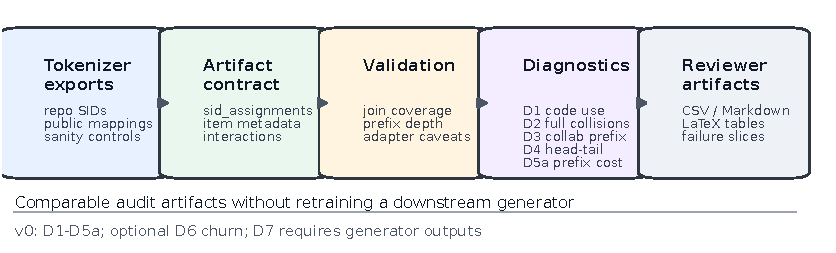
\includegraphics[width=\columnwidth]{figures/fig1_audit_sid_pipeline.pdf}
\caption{\tool normalizes heterogeneous \sid exports through a mapping-first
contract and reports D1--D5a diagnostics. The bottom panels preview
representative outputs from the Musical case study and controllers: capacity
pressure, full-code collisions, collaborative-prefix recovery, head-tail
allocation, and realized prefix cost. D6 is optional churn evidence; D7
requires generator outputs or beam traces.}
\Description{Pipeline plus diagnostic preview. A top row shows SID artifact,
adapter, validator, D1-D5a reports, and audit tables. Four small panels show
capacity/collision, collaborative prefix recovery, head-tail capacity, and
prefix-cost boundary examples.}
\label{fig:audit-sid-pipeline}
\end{figure}

\paragraph{Artifact contract.}
The required contract has three checks: each row has a stable item key, every
\sid level is a discrete token, and the diagnostic item universe is joinable to
metadata and interaction slices. Metadata enables semantic/category slices;
interactions enable collaborative-neighborhood and head-tail diagnostics. The
\texttt{generator\_outputs} table is optional because many public tokenizer
releases expose item codes without trained generator traces.

\paragraph{Evidence roles.}
\tool separates rows by what they can support. A named-method row comes from a
public method path and can support method-facing artifact claims. A controlled
stressor is deliberately synthetic or method-inspired and can test whether a
diagnostic reacts to a mechanism, but it is not method coverage. Optional rows
exercise extensions such as drift or non-Amazon schemas. Literature-only rows
motivate the design space but are not loaded as runnable evidence.

\paragraph{Validation before metrics.}
Adapters are refused as evidence until they pass item-count agreement,
missing-code, duplicate-key, depth-consistency, and provenance checks. This
guard is necessary because public SID repositories may expose checkpoints, item
mappings, codebooks, intermediate feature files, or only partial releases. The
manifest records each row's evidence role and caveats before any D1--D7 number
is emitted.

Prior recommender resources such as RecList and Elliot motivate diagnostic and
reproducible evaluation beyond a single aggregate metric~\cite{chia2022reclist,anelli2021elliot}.
\tool applies that resource logic to a newer artifact boundary: the item
address space consumed by generative recommenders.
